% !BIB TS-program =
\documentclass{svproc}
\usepackage{url}
\usepackage{graphicx}
\usepackage{amsmath}
\usepackage{algorithm}
\usepackage[noend]{algpseudocode}
\def\UrlFont{\rmfamily}
\tolerance=1
\emergencystretch=\maxdimen
\hyphenpenalty=10000
\hbadness=10000

\begin{document}
\mainmatter
\title{Analysis of different AI Strategies for Solving Picross Puzzles}
\subtitle{CS7IS2 Project (2020/2021)}
\author{Andrej Liadov, Edvinas Teiserskis, Min Wu, Edmond Cheng, Adam McQuade}
\authorrunning{A. Liadov, E. Teiserskis, M. Wu, E. Cheng, A. McQuade}
\institute{
  \email{liadova@tcd.ie}, \email{teiserse@tcd.ie}, \email{wumi@tcd.ie}, \email{chenge@tcd.ie}, \email{amcquade@tcd.ie}}

\maketitle              % typeset the title of the contribution


\begin{abstract}
Research in Artificial Intelligence has always had a very strong relationship with games and game-playing. Picross (a.k.a nonograms) are logic puzzles with simple rules and challenging solutions, and in this case our research provides a survey that analyses and compares different AI algorithms - uniform cost search, Q-learning, constraint satisfaction problems (CSPs) and genetic algorithms (GA) applied to solve picross puzzles. Through the process of implementation and evaluation we analyse there algorithms and find out their common aspects, differences, connections between methods, drawbacks and open problems.
\keywords{artificial intelligence, uniform cost search, Q-learning, CSPs, Genetic Algorithms}
\end{abstract}


\section{Introduction}
Artificial intelligence (AI) is the emulation of human intelligence of computers that are designed to think and behave like humans. As AI has evolved to have a huge global influence, it operates by integrating vast volumes of data with quick, iterative analysis and intelligent algorithms, which enables the program to learn automatically from patterns or features in the data.

Picross, also known as Nonograms, is a logic puzzle in which the player uses provided rules to mark (or omit from marking) cells in a grid. Typically, the rules are given as lists of numbers at the sides of the grid (see Figure 1). As these puzzles (typically) have only one solution, the best method to solve them is determined by the speed of the solution. However, playing games like a human is other than thinking about games like a human or learning like one. There is a famous saying that game-playing is the Drosophila of AI. And yet in our research it could be that the task of playing picross, once it’s converted into the task of searching some certain nodes evaluated by time consumed, it is also a different kind of intelligence.

\begin{figure}[h]
  \centering
  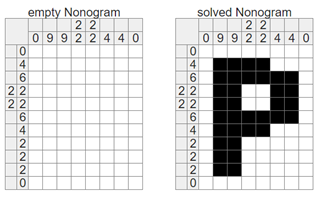
\includegraphics[width=0.6\textwidth]{picross1.png}
  \caption{An example of a picross puzzle, with the start state on the left and completed puzzle on the right. The numbered hints describe how many contiguous blocks of cells are filled. Black cells mark filled cells and blank cells mark unfilled cells. Example from \texttt{https://en.wikipedia.org/wiki/Nonogram}, sourced 2021-04-28.}
\end{figure}

Our goal is to analyse the solving of picross puzzles, and determine which is the best among the 4 approaches we are examining. These types of results can be used for picross design feedback, content generation, or difficulty estimation. One potential use is in order for humans to use these computer-generated strategies, the strategies must be both efficient in the domain of interest and concisely articulated so that a designer can consider the whole strategy in their head. For example, there are dozens of documented strategies for picross\cite{picross1}, and puzzle designers construct puzzles and rank their difficulty based on which of these strategies are used\cite{picross2}.

This paper presents a comparison of 4 different AI algorithms - uniform cost search, Q-learning, CSP and GA - that we  have decided to apply to solving picross puzzles. The paper also evaluates these algorithms based on their execution time, memory usage and other metrics. Through the process of implementation and evaluation we show the pros and cons of each algorithm, and we also examine their common aspects and differences, connections between methods, drawbacks and open problems. Our recording of presentation link of this research is xxx.


\section{Related Work}
Picross, like other logic puzzles such as Sudoku, has special answers which can be solved by deducing pieces of the answer in any order. In Sudoku, the squares are filled with one number each while in Picross each square is either filled in or left blank. Prior work has also examined the solutions of logic puzzles, but most existing solvers are programs written from scratch for the express purpose of solving paint-by-number puzzles\cite{5.1.1,5.1.2,5.1.3,5.1.7}. Browne provides a deductive search algorithm that is intended to mimic the constraints and method of human solvers\cite{Browne}. The complexity of picross can be estimated by calculating the number of steps that can be solved one row/column at a time according to Batenburg and Kosters\cite{Batenburg and Kosters}.

Heuristic search is a technique that uses a heuristic value for optimizing the search. Many heuristic solving steps are given in order to determine the value of some pixels in a single row or column\cite{Salcedo}, and in order to decide which pixels can be assigned a certain value that they use run ranges\cite{CHYU}. The methodology behind is to assign an integer range to each row or column description, the lowest and largest pixel number can be used to contain the run’s black pixels corresponding to the definition of the integer. An example of applying heuristic steps to fill the pixels is Teal’s Nonogram Solver\cite{Teal}, the input for this solver is given by a single string containing the row and column definitions one by one. In other words, this solver runs through all rows and columns one by one, while applying heuristic steps in order to fill pixels. However, the solver leaves several pixels undetermined, which can clearly be filled by logic decisions. These are pixels that need input from the last pixels in a run, usually at the end of a row or column. Based on this, we will choose GA to solve the picross puzzles because as GA is a class of heuristic optimization methods, it mimics the process of natural evolution by modifying a population of individual solutions which makes it easier to achieve our goal. A-star is another heuristic algorithm that is commonly used in pathfinding and graph traversal, which is the method of mapping an easily traversable path between multiple nodes\cite{astar}.

The Backtracking Heuristic (BH) methodology consists in to construct blocks of items by combination between heuristic, that solve mathematical programming models, and backtrack search algorithm to figure out the best heuristics and their best ordering\cite{BH}.

Backtracking Search for CSP: Some hobbyists have created programs that solve Sudoku puzzles using a backtracking algorithm, which is a form of brute force search\cite{brute}. Backtracking is a depth-first search (as comparison to a breadth-first search) so it can completely investigate one branch to a potential solution before going on to another. A brute force algorithm visits the empty cells in some order, filling in digits sequentially, or backtracking when the number is found to be not valid\cite{Peter,lecture}.

Reinforcement Learning for CSP: According to \cite{Qlearning}, the constraints could be presented as an image, and hence Mehta chose the algorithm used for Sudoku to be Deep Q-Learning. The Q agent is trained with no rules of the game, with only the reward corresponding to each state's action. This paper\cite{Qlearning} contributes to choosing the reward structure, state representation, and formulation of the deep neural network.

Genetic algorithms have found much use in puzzle-based problem solving. According to \cite{geneticAlgo}, genetic algorithms are well suited for multi-objective optimisation problems, such as sudoku puzzles. Search algorithms are a commonly deployed in games to find an optimal solution to a problem with many path options. A problem encountered by search algorithms is the high time and space complexities required when the search domain becomes exceedingly large. Genetic algorithms are a way of mitigating this downside of search algorithms with respect to solution searching, and have been demonstrated as effective in solving other constraint based puzzles such as sudoku.

A genetic algorithm is a stochastic optimization algorithm. It takes inspiration from biological ideas such as the theory of evolution put forth by Charles Darwin. In this theory, genetic characteristics are passed down through successive generations following successful reproduction. Successful production of offspring is dependent on many factors, including the suitability of the parents to the local environment. When applied to optimisation algorithms, parents may be thought of as an instance of an agent attempting to reach a goal. A generation is a population of these instances with slight differences between their characteristic parameters. Following each iteration of the agents attempting to reach a goal state, the agents with the best progress are given a higher probability of producing offspring. The next generation is produced as a function of this probability. Thus, each cohort of agents is a slight modification of the previous population, weighted towards the most successful members of the previous generation. Over many iterations, the population should become optimized to the environment, thus having more success in reaching the goal state.



\section{Problem Definition and Algorithm}
This section formalises the problem you are addressing and the models used to solve it. This section should provide a technical discussion of the chosen/implemented algorithms. A pseudocode description of the algorithm(s) can also be beneficial to a clear explanation. It is also possible to provide one example that clarifies the way an algorithm works. It is important to highlight in this section the possible parameters involved in the model and their impact, as well as all the implementation choices that can impact the algorithm.

\subsection{Uniform Cost Search}
We have implemented an uniform cost search solution to solve picross puzzles - while this is an established search algorithm, this requires our problem to be represented as a searchable graph.

We did this by modelling the puzzle as a graph - The start state is an empty puzzle, and the next states are potential moves of filling in a square as a particular colour, out of all unfilled squares (our only factor of filtering is if a row/column combination allows for a colour). The cost function we have implemented is looking at the row/column of the square in question, and calculating:

$$ (1 - row_{proportion}) * (1 - column_{propotion}) $$

where $row/column_{proportion}$ is the number of squares of that colour in that row/column divided by the height/width of the puzzle. As such, in the intersection of a full row/column pair, the action cost is zero, of a nearly full pair close to zero and for a sparse pair approaching one. This gives us a cost function which makes cheaper locations that will be more likely to contain a square of that colour.

While the original plan was to add onto this a heuristic in order to implement a-star search, we could not come up with a sensible way to derive a heuristic from the state of the puzzle - either we would produce a calculation that would most likely not correspond to a useful way to estimate the "completeness" of a puzzle, or we would effectively be encoding another method like constraint programming within the heuristic itself (making the surrounding search implementation redundant).

Due to the nature of the puzzle, using search is expected to be the worst performing method, and is mainly created as an example. Since the puzzle can have an inordinate number of states, and there is a massive expansion of state transitions at each state, using a search approach immediately hits major speed and memory limits.

For example, taking a monochrome 5x5 puzzle, we have $2^{25}$ total possible states, and most states have a numerous amount of state transitions - 25 from the initial state, 24 from \textit{each} state following those, and so on. As such, the frontier of the search grows at a very rapid pace - this both makes each state take additional computing time, and quickly fills up the physical limits of available memory on most computers.

Some reduction occurs from the fact that the cost and result of two paths leading to the same state are regardless of order, allowing us to collapse in duplicate entries. However, this does not nearly reduce the load of the approach to a state where is it comparable to other methods that actively check against the puzzle's rules and full current state in a sensible manner.

\subsection{Q-Learning}
First the state space and the actions space had to be defined for the problem in order to create a Q-learning agent. 

The state of a given puzzle was defined as the the rows that were filled in by the Q-leaning agent. If there were different permutation chosen for a given row of a given puzzle, the state of the puzzle would be different.

The action space for a given puzzle would be defined by getting the permutations of the row that are left to be filled in. Choosing a row to fill would be considered an action that would consequently move the agent to a different state. If an action is chosen for a row it is not possible to reverse that action. The row would be filled if an action was taken and as a result, there would not be any actions available for that row.

The state space contains two methods of exiting the puzzle. The first method is to fill in all rows the to not have any more actions to take. If there are no more actions to take, the algorithm checks whether the solution to the puzzle is correct. If the answer to the puzzle is correct, the reward returned is 1000. If the completed puzzle is incorrect, the reward returned is -100.

Q-learning with a q-table is meant to choose actions in such a way that the reward is maximised. The state space contains very few solutions. In most of the puzzles tested there was a unique correct solution, in some cases there might have been several solutions. That means that the correct solution space is extremely sparse while the incorrect solution space is quite vast. The contrast between correct solution space and incorrect solution space was reflected in the calculation of reward. Taking an action that did not complete the puzzle should always result in a reward of +1. If the an action taken results in a correct solution, a reward returned was +1000 and if the solution was incorrect, a reward of -100 was returned.

The approach to exploration was a soft-max approach. The exploration rate \epsilon would be high very high to begin with because nothing is known about the reward, action and state space. A high \epsilon encourage the agent to choose random actions. A random number is generated between [0-1] and if epsilon is larger than the the random number, the agent picks a random action. If not, it picks the action with the highest q-value. Epsilon has a pre-defined decay rate. By the time the episode number reaches 100, the agent should be a hard-max solver, meaning the agent only picks the best q-value.

The number of episodes will determine how many times the problem will be solved and as a result the q-table will be updated in a proportional amount since the q-table will be updated after every action. The pseudo-code for an episode is given below.

\begin{algorithm}
    \caption{Q-Learning Algorithm}\label{euclid}
    \begin{algorithmic}[1]
    	\For {$\textit{episode} in \textit{num_episodes}$}
    		\State $\textit{agent.puzzle} = \textit{read_puzzle()}$
    		\For {$\textit{step} in \textit{max_steps}$}
    			\If {$agent.is_explore()$}
    				\State $\textit{action = agent.get_random_action()}$
    			\EndIf
    			\Else
    				\State $\textit{action = agent.get_action()}$
    			\EndElse
    			\State $\textit{new_state, reward, complete = agent.step(action)}$
    			\State $\textit{agent.update_qtable(action, new_state, reward)}$
    			\State $agent.puzzle = new_state.puzzle$
    			\If{$complete$}
    				break
    			\EndIf
    		\EndFor
    	\EndFor
    \end{algorithmic}
\end{algorithm}

Updating the q-table is done the Bellman equation. This process is done by combined the old q-value with a learning rate, the reward, the discount rate and the max q-value in the future state. The equation is given below. Alpha is the learning rate and it determines how much influence the new q-value will have on the old one. The higher the learning rate, the more influence the future q-value will have.

\begin{equation}
	NewQ(s, a) = (1 - \alpha)Q(s,a) + \alpha[R(s,a) + \gamma maxQ'(s', a') - Q(s,a)] 
\end{equation}

\subsection{Constraint Programming}
The basis of the constraint programming algorithm applied was backtracking, with constraint propagation. Depth first search was used as the backend to apply backtracking. The algorithm starts off with an empty puzzle. All permutations of the first row are generated and filtered. The filtering process here refers to  constraint propagation. Constraint propagation is applied as follows:

\begin{enumerate}
    \item Generate all permutation of row
    \item For each row, check if the column constraint is broken. A column constraint is broken when that column does not contain that colour.
    \item Return list of all feasible rows
\end{enumerate}

The returned list of rows is used to set the states of the backtracking algorithm. Every time a row is set into the nonogram puzzle, the state of the nonogram is checked. Every column in the puzzle is checked. If the number of occurrences of any given colour is greater than the what the constraints dictate, then that row is removed. Figure \ref{fig:Backtrack} below displays this process. This checking is done every time a new row is added.

\begin{figure}[h]
    \centering
    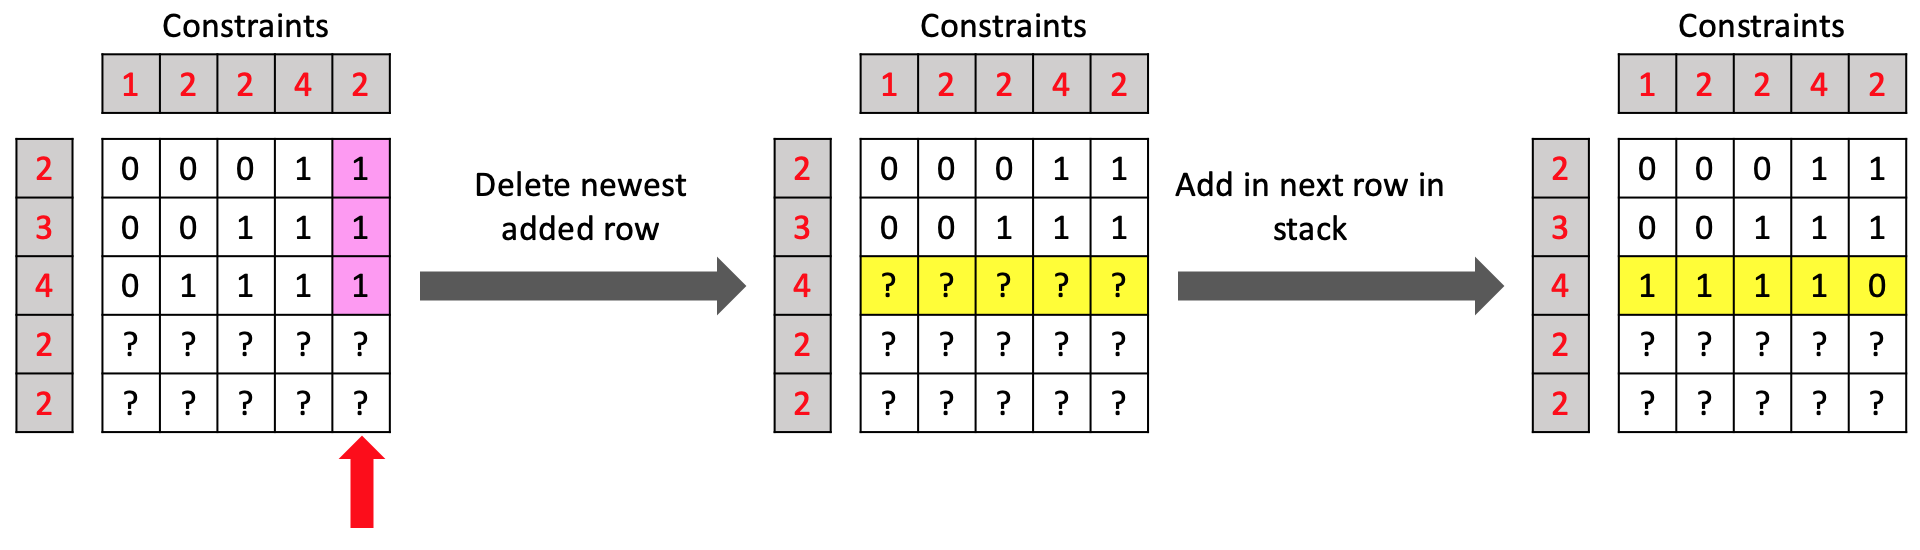
\includegraphics[scale=0.36]{Backtracking.png}
    \caption{Backtracking}
    \label{fig:Backtrack}
\end{figure}

The overall algorithm is shown below.

\begin{algorithm}
    \caption{CSP Algorithm}\label{euclid}
    \begin{algorithmic}[1]
        \State $\textit{stack} = \text{LIFO\_stack}$
        \State $\textit{all\_rows} = \text{generate\_all\_rows[row\_index]}$
        \State $\textit{viable\_rows} = \text{filter\_rows(all\_rows)}$
        \While {$\textit{stack } \text{!= } \textit{empty}$}
        \State $\textit{row} = \text{stack.pop}$
        \State $\text{puzzle.insert\_row(row)}$
        \State $\textit{check} = \textit{puzzle.check\_constraints}$
        \If {$check == False$}
        \State $\text{puzzle.delete\_row(row)} \to \text{continue}$
        \EndIf
        \While {$\textit{index} < \textit{puzzle.height}$}
        \State $\textit{stack.push(generate\_all\_rows(index)}$
        \EndWhile
        \EndWhile
    \end{algorithmic}
\end{algorithm}

\subsection{Genetic Algorithms}
The approach taken in this project follows the typical genetic algorithm design implementation. The programme reads the rules file which determines the constraints for each nonogram puzzle.

Selection: the parents for the next generation are selected based on a metric known as fitness. In this implementation, fitness is a measure of how many of the constraints are left unsatisfied by a parent solution. The agents are sorted by those with the lowest number of unsatisfied constraints and these are more likely to be parents.

Crossover: is the process of combining the characteristics of two parents to form a child. Using a probability function, a random split of each of two parents characteristics is taken and recombined into a new characteristic. This is undertaken for each pair of parents at the end of an iteration to create the new generation.

Mutation: this is the process of randomly altering minor details in the characteristics of the new generation of agents. In this case it implies that a random block within the nonogram will be flipped from filled to unfilled.

\section{Experimental Results}
	This section should provide the details of the evaluation. Specifically:
\begin{itemize}
	\item Methodology: describe the evaluation criteria, the data used during the evaluation, and the methodology followed to perform the evaluation.
	\item Results: present the results of the experimental evaluation. Graphical data and tables are two common ways to present the results. Also, a comparison with a baseline should be provided.
	\item Discussion: discuss the implication of the results of the proposed algorithms/models. What are the weakness/strengths of the method(s) compared with the other methods/baseline?
\end{itemize}


\section{Conclusions}
Provide a final discussion of the main results and conclusions of the report. Comment on the lesson learnt and possible improvements.

A standard and well formatted bibliography of papers cited in the report. For example:

\begin{thebibliography}{6}

\bibitem {Browne}
Cameron Browne. 2013. Deductive search for logic puzzles. In Computational
Intelligence in Games (CIG), 2013 IEEE Conference on. IEEE.

\bibitem {Batenburg and Kosters}
K Joost Batenburg and Walter A Kosters. 2012. On the difficulty of Nonograms.
ICGA Journal 35, 4 (2012), 195–205.

\bibitem {5.1.1}
Jan Wolter's pbnsolve Program
\url{https://webpbn.com/pbnsolve.html}

\bibitem{5.1.2}
Mirek and Petr Olšák's Nonogram Solver
\url{http://www.olsak.net/grid.html#English}

\bibitem{5.1.3}
Steve Simpson's Nonogram Solver
\url{http://www.comp.lancs.ac.uk/~ss/software/nonowimp/}

\bibitem{5.1.7}
Jakub Wilk's Nonogram Solver
\url{http://jwilk.nfshost.com/software/nonogram.html}

\bibitem{Teal}
\url{http://a.teall.info/nonogram}

\bibitem{Salcedo}
S. Salcedo-Sanz, E.G. Ort’iz-Garc’ia et al., Solving Japanese Puzzles with
Heuristics, IEEE Symposium on Computational Intelligence and Games,
2007, 224-231, CIG, 2007.

\bibitem{CHYU}
C.H. Yu, H.L. Lee, L.H. Chen, An efficient algorithm for solving nonograms, Springer Science+Business Media, Springer Verlag, Applied Intelligence 35(1): 18-31, 2011

\bibitem{Peter}
Norvig, Peter. "Solving Every Sudoku Puzzle". Peter Norvig (personal website). Retrieved 24 December 2016.
\url{http://www.norvig.com/sudoku.html}

\bibitem{lecture}
Zelenski, Julie (July 16, 2008). Lecture 11 | Programming Abstractions (Stanford). Stanford Computer Science Department.
\url{https://www.youtube.com/watch?v=p-gpaIGRCQI}

\bibitem{brute}
Brute Force Search, December 14th, 2009.
\url{http://intelligence.worldofcomputing/brute-force-search}

\bibitem{picross1}
Andrew C Stuart. 2007. The Logic of Sudoku. Michael Mepham Publishing.

\bibitem{picross2}
Andrew C Stuart. 2012. Sudoku Creation and Grading. (January 2012).
\url{http://www.sudokuwiki.org/Sudoku Creation and Grading.pdf}
[Online, accessed 8 Mar 2017].

\bibitem{Qlearning}
Mehta, Anav. "Reinforcement Learning For Constraint Satisfaction Game Agents (15-Puzzle, Minesweeper, 2048, and Sudoku)." arXiv preprint arXiv:2102.06019 (2021).

\bibitem{astar}
Solving 8-Puzzle using A* Algorithm
\url{https://blog.goodaudience.com/solving-8-puzzle-using-a-algorithm-7b509c331288}

\bibitem{geneticAlgo}
Using genetic algorithms to solve sudoku puzzles
\url{https://ieeexplore.ieee.org/document/4424632}

\bibitem{BH}
Jonatã L., Araújo P., Pinheiro P.R. (2011) Applying Backtracking Heuristics for Constrained Two-Dimensional Guillotine Cutting Problems. In: Liu B., Chai C. (eds) Information Computing and Applications. ICICA 2011. Lecture Notes in Computer Science, vol 7030. Springer, Berlin, Heidelberg.

\end{thebibliography}

\end{document}
